\documentclass[serif,compress, blue, 11pt]{beamer}
\mode<presentation>
\usetheme{Warsaw}
\useoutertheme[subsection=false]{smoothbars}

% include packages
\usepackage{subfigure}
\usepackage{multicol}
\usepackage{amsmath}
\usepackage{epsfig}
\usepackage{graphicx}
\usepackage[all,knot]{xy}
\xyoption{arc}
\usepackage{url}
\usepackage{multimedia}
\usepackage{hyperref}
\usepackage{setspace}
\graphicspath{{~/Documents/ipm/Doklad/2014/yschool2014}}
%\usepackage[utf8x]{inputenc}
\usepackage[utf8x]{inputenc}
\usepackage[english,russian]{babel}

\setbeamerfont{frametitle}{size=\small}


\title[Scientific School for Young Scientists, 2014]{\textbf{Modeling~flow~in~a~viscous\\~
continuously~stratified~fluid~taking\\~into~account~diffusivity~effects}}
\author[Alexey Vasiliev, IPMEch RAS, Russia]{%
  Vasiliev~Alexey}
\institute[Institute for Problems in Mechanics of the RAS]{Laboratory of Fluid Mechanics\\
  Institute for Problems in Mechanics of the RAS\\
  Moscow, Russia
  }
\date[ 2014]{Firth International Scientific School for Young Scientists. \\"Waves and vortices in complex media", 2014}

\begin{document}

\frame{
	\titlepage
}

\section[Into]{}

\section{Motivation}


\subsection{Review}
\frame{\frametitle{Review}
\begin{enumerate}
\item J.V.S. Rayleigh
\item J. Lighthill 
\item Yu.D. Chashechkin 
\item V.A. Gorodtsov 
\item T.N. Stevenson 
\item D.G. Hurley, G.J. Keady 
\item B.R. Sutherland 
\item Yu.V. Kistovich  
\item A.V. Kistovich 
\item B. Voisin 
\end{enumerate}
}

\subsection{Color schlirien images oscillation of disk}
\frame{\frametitle{Color schlirien images oscillation of disk}
\begin{figure}
\center 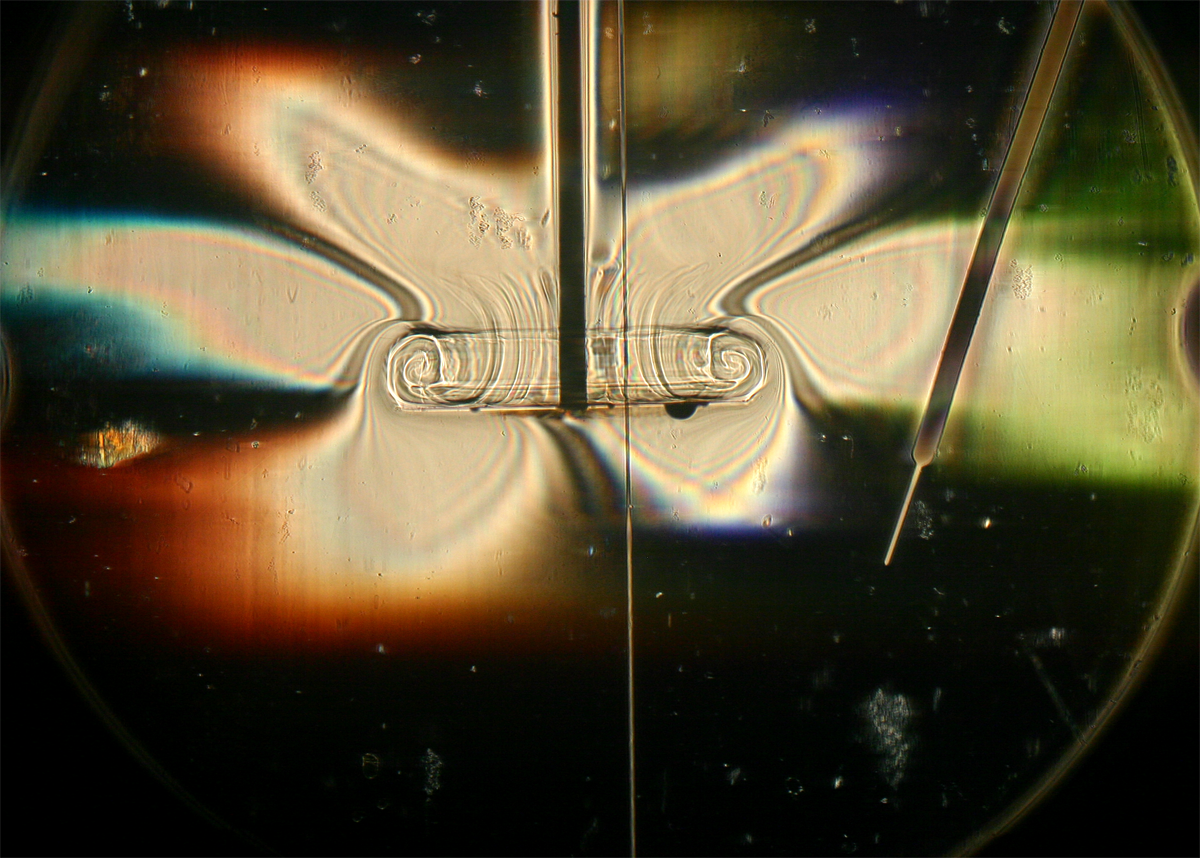
\includegraphics[width=0.7\linewidth]{disk1.png} 
\end{figure}}



\section{Math. model}
\subsection{System coordinate frame}
\frame{\frametitle{System coordinate frame for analytical analyze}
\begin{figure}
   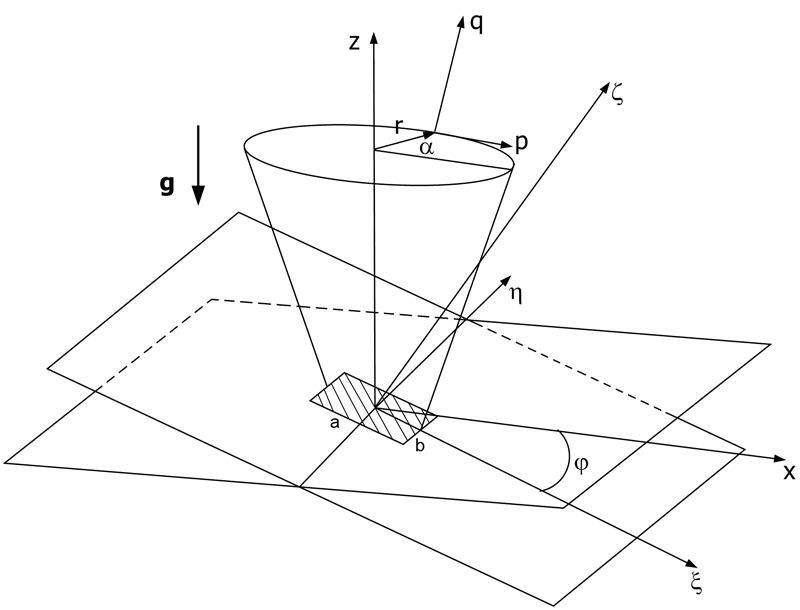
\includegraphics[width=0.8\linewidth]{sys-coord.png}
\end{figure}
}

\subsection{Governing equations and boundary conditions}
\frame{\frametitle{Governing equations and boundary conditions}
\textbf{Governing equations}
\[
\frac{{\partial \rho} }{{\partial t}} + \textbf{v} \nabla \rho = 0,
\quad
\operatorname{div}\; \textbf{v} = 0
\]
\[
\frac{{\partial \textbf {v}} }{{\partial t}} + \left( {\textbf{v},\nabla} \right) \textbf{v} = \frac{1}{\rho} \nabla p + \nu \Delta v + \rho \textbf{g}
\]
\[
\frac{{\partial S} }{{\partial t}} = \kappa_S \Delta S + \frac{v_z}{\Lambda} 
\]
\textbf{Boundary conditions}
\[
\left. {\textbf{v}} \right|_{\Gamma}  = \textbf{u}_{0} e^{ - i\omega t},
\quad
\kappa _{S} \left. {\frac{{\partial S}}{{\partial n}}} \right|_{\Gamma}  = 0
\]

\[
 v \to 0,
\quad
\rho \to \rho _{0} ,
\quad
{{\partial P} \mathord{\left/ {\vphantom {{\partial P} {\partial z}}} 
\right. \kern-\nulldelimiterspace} {\partial z}} \to \rho _{0} \left( {z} 
\right)g, r \to \infty
\]


\textbf{Toroidal-poloidal decomposition}
\[
\textbf{v} = 
\nabla \times \textbf{e}_{z} \Phi + \nabla \times \left( {\nabla \times \textbf{e}_{z} \Psi}  
\right)
\]

}

\frame{\frametitle{System equations for functions $\Phi$ and $\Psi$}
\[
\left( {\left( {\frac{{\partial} }{{\partial t}} - D\Delta}  \right)\left( 
{\frac{{\partial} }{{\partial t}} - \nu \Delta}  \right)\Delta + N^{2}\Delta 
_{ \bot} }  \right)\;\Phi = 0
\]

\[
\left( {\frac{{\partial} }{{\partial t}} - 
\nu \Delta}  \right)\;\Psi = 0
\]

\[
\left( {\left( {\frac{{\partial} }{{\partial t}} - D\Delta}  \right)\left( 
{\frac{{\partial} }{{\partial t}} - \nu \Delta}  \right)\Delta + N^{2}\Delta 
_{ \bot} }  \right)\;S = 0
\]

where 
\[
\Delta _{ \bot}  = \partial _{x} ^{2} + \partial _{y} ^{2} 
\quad
\Delta  = \partial _{x} ^{2} + \partial _{y} ^{2} +\partial_{z}^2
\quad
N^2=\sqrt{\frac{g}{\Lambda}}
\]
}


\frame{\frametitle{Construction solution for $\Phi$ and $\Psi$ in Fourier transform}
\[
\Phi = e^{ - i\omega t}\sum\limits_{j = 1}^{3} {\int\limits_{ - \infty} ^{ + 
\infty}  {A_{j} \left( {k_{\xi}  ,k_{\eta} }  \right)E_{j} \;dk_{\xi}  
dk_{\eta} } }
\]

\[
S = - \frac{{\rho _{0}} }{{\Lambda} }e^{ - i\omega t}\sum\limits_{j = 1}^{3} 
{\int\limits_{ - \infty} ^{ + \infty}  {\frac{{\left( {k_{\xi}  \cos\varphi - 
k_{j} \sin\varphi}  \right){}^{2} + k_{\eta}  {}^{2}}}{{i\omega - \kappa _{S} 
\;k^{2}}}A_{j} \left( {k_{\xi}  ,k_{\eta} }  \right)}}  E_{j} dk_{\xi}  
dk_{\eta}
\]

\[
\Psi = e^{ - i\omega t}\int\limits_{ - \infty} ^{ + \infty}  {B\left( 
{k_{\xi}  ,k_{\eta} }  \right)\;E_{4} dk_{\xi}  dk_{\eta} }
\]

where

\[
E_{j} = \exp\left( {ik_{j} \zeta + ik_{\xi}  \xi + ik_{\eta}  \eta}  \right),
\quad
k = \sqrt {k_{j}^{2} + k_{\xi} ^{2} + k_{\eta} ^{2}}
\]

}

\section{Theoretical analyze}
\subsection{Viscous stratified fluid take into diffusion}
\frame{\frametitle{Viscous stratified fluid take into diffusion}
\textbf{Dispersion equation}
\[
\left( {\nu \kappa _{S} \tilde {k}^{6} - i\omega \left( {\nu + \kappa _{S}}  
\right)\tilde {k}^{4} - \omega ^{2}\tilde {k}^{2} + N^{2}k_{ \bot} ^{2}}  
\right) \left( \tilde{k}^{2} + \frac{\omega}{i\nu} \right) = 0
\]

\[
\tilde {k}^{2} = 2k_{\zeta} ^{2} + k_{ \bot} ^{2} ,
\quad
k_{ \bot} ^{2} = k_{\xi} ^{2} + k_{\eta} ^{2} 
\]
}

\frame{\frametitle{Viscous stratified fluid take into diffusion}
\textbf{Regular solution(waves)}
\[
 k_{1} = \frac{{k_{\xi}  \sin\varphi \cos\varphi \pm \kappa \cos\theta} }{{\mu_{\theta}} } 
\pm \delta _{N}^{2} \left( {1 + \varepsilon}  \right)\frac{{i\; \tan\theta \mu_{\theta}^{4}}}{{2\kappa \mu 
^{4}}} + ...
\]

\[
\mu = \sin^{2}\varphi - \sin^{2}\theta,
\quad
\mu_{\theta} = \left({k_{\xi}  \sin\varphi \cos\varphi \pm \kappa \cos\varphi}  \right),
\]
\[
 \varepsilon = Sc^{ - 1} = \frac{{\kappa _{S}} }{{\nu} },
\quad
 \delta _{N} = \sqrt {\frac{{\nu} }{{N}}} 
\]

\textbf{Singular solution} \\
\[
k_{2,\;3} \approx \sqrt {\frac{{i\omega \left( {\varepsilon + 1 \pm \lambda 
_{\nu \kappa} }  \right)}}{{\varepsilon} }} ,
\quad
\lambda _{\nu \kappa}  = \frac{{2}}{{\sin\theta} }\sqrt {\left( {1 + 
\varepsilon}  \right)^{2} - \frac{{4\varepsilon \mu} }{{\sin^{2}\theta} }}
\]

\vspace{0.25cm}

\[
 k_{4} = \sqrt {\frac{{2i}}{{\delta _{\nu} ^{2}} } - k^{2}},
\quad
\delta _{\nu}  = \delta _{N} \sqrt {\frac{{2}}{{\sin\theta} }} ,
\quad
\delta _{\varphi}  = \delta _{N} \sqrt {{\textstyle{{2\sin\theta}  \over {\left| 
{\mu}  \right|}}}},
\quad
\delta _{\kappa}  = \delta _{N} \sqrt {{\textstyle{{2\varepsilon}  \over 
{\sin\theta} }}}
\]


}

\frame{\frametitle{Viscous stratified fluid take into diffusion.Vetrical component of the velocity}

\[
v_{\zeta} \approx \int\limits_{ - \infty} ^{ + \infty}  {A_{1} \left( 
{k_{\eta} ^{2} \sin\varphi - k_{\xi}  \beta _{1}}  \right)E_{1} dk_{\xi}  dk_{\eta} }  -
\]


\[
- ie^{\frac{{i - 1}}{{\delta _{\nu} } }\zeta 
}\sin\varphi \int\limits_{ - \infty} ^{ + \infty}  {B E_{\xi \eta} \;dk_{\xi}  dk_{\eta} }  -
\frac{{i + 1}}{{\delta _{\varphi 
}} }e^{\frac{{i - 1}}{{\delta _{\varphi} } }\zeta} \cos\varphi \int\limits_{ 
- \infty} ^{ + \infty}  {A_{2} k_{\xi}  E_{\xi \eta} dk_{\xi}  dk_{\eta} } -
\]

\[
 - \frac{{1 + i}}{{\delta _{\kappa} } }\sqrt {\frac{{\sin\theta} }{{2}}} e^{ 
- \frac{{\sqrt {\sin\theta} } }{{\delta _{\kappa}  \sqrt {2}} }\zeta + 
\frac{{i\zeta} }{{\delta _{\kappa}  \sqrt {2}} }}\cos\varphi \int\limits_{ - 
\infty} ^{ + \infty}  {A_{3} k_{\xi}  E_{\xi \eta} dk_{\xi}  dk_{\eta} }
\]

where 
\[
E_{\xi \eta} = exp\left( {ik_{\xi}  \xi + ik_{\eta}  \eta} \right)
\]
}

\subsection{Comparison theoretical analyze and measurement.}
\frame{\frametitle{Comparison theoretical analyze and measurement. Source is disk $u_{0}=0.25 cm\ s^{-1}$}
\begin{figure}
\begin{minipage}{0.47\linewidth}
 \center{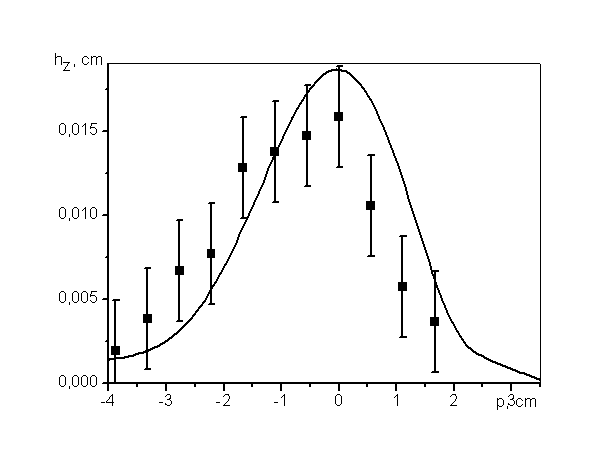
\includegraphics[width=0.95\linewidth]{theory-experim-1.png}}\\
\tiny{$R=1.75$ cm, $N=1.0\ s^{-1}$, $\omega=0.57\ s^{-1}$}
\end{minipage}
\begin{minipage}{0.47\linewidth}
 \center{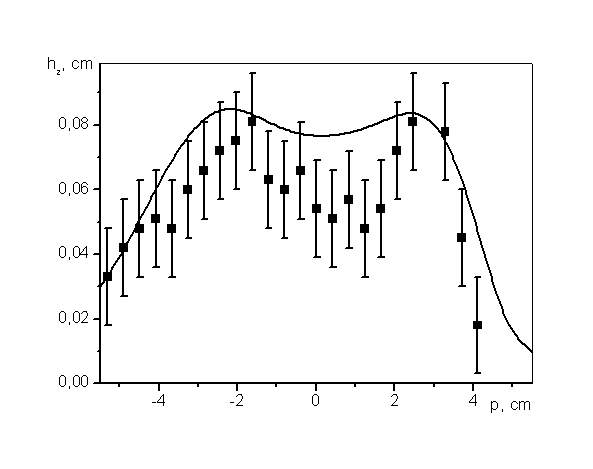
\includegraphics[width=0.95\linewidth]{theory-experim-2.png}}\\
\tiny{$R=4.0$ cm, $N=1.26\ s^{-1}$, $\omega=1.11\ s^{-1}$}
\end{minipage}
\end{figure}
}

\section{Numerical analyze}

\subsection{Why OpenFOAM?}
\frame{\frametitle{Why OpenFOAM?}
\textbf{Pluses:}
\begin{enumerate}
\item OpenFOAM free and open source, under the GNU general public licence (GPL). 
%The GPL gives users the freedom to modify and redistribute the software and a guarantee of continued free use - 
%as long as the terms of the GPL are adhered to.
\item Support of community 
{\bf http://www.cfd-online.com/Forums/openfoam/}, {\bf http://openfoamwiki.net/}
\item Support open-source Linux platform (openSUSE, Ubuntu, Fedora and etc)
\end{enumerate}
\textbf{Minuses:}
\begin{enumerate}
\item OpenFOAM has no GUI to create grids, but can use other applications such as:
GMSH ({\bf http://geuz.org/gmsh/}), Salome ({\bf http://www.salome-platform.org/}) or commercial mesh generators such as:
Icem CFD ({\bf www.ansys.com}), Gambit ({\bf www.ansys.com}), pro*star Star-CD ({\bf www.cd-adapco.com})
\end{enumerate}
}

\subsection{WF process for analyze and solving}
\frame{\frametitle{Hardware, software and workflow process for analyze and solving}
\begin{figure}
\center 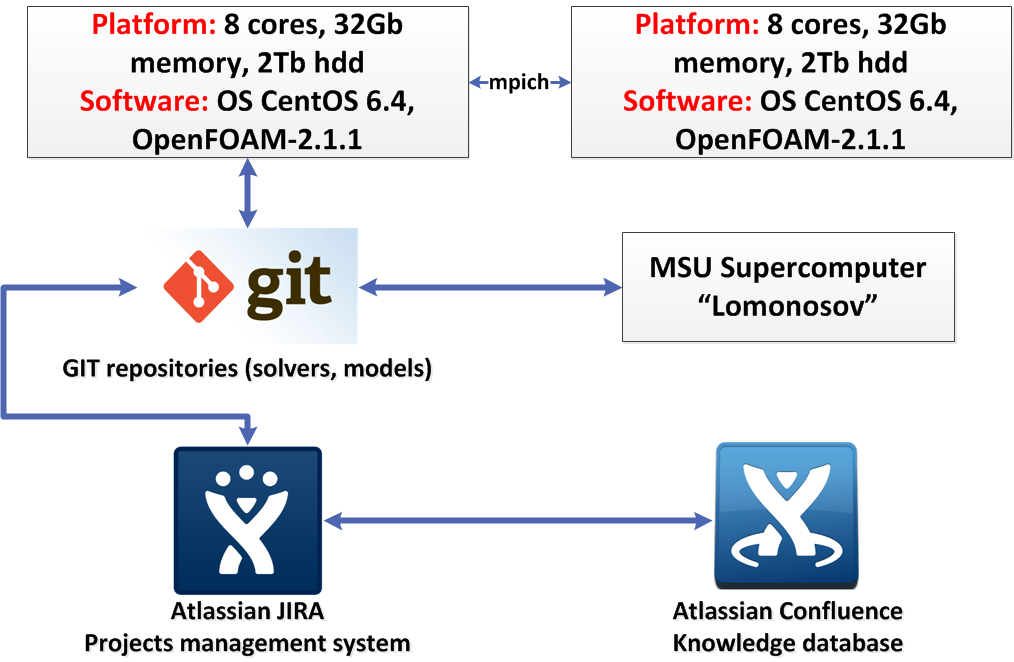
\includegraphics[width=0.95\linewidth]{scheme-openfoam-jira-confluence.png} 
\end{figure}
}

\subsection{IGWFoam.C}
\begin{frame}[fragile]\frametitle{Structure of the solver. IGWFoam.C}
\begin{block}{Navier - Stokes equations}
\begin{verbatim}
   fvVectorMatrix UEqn (
      fvm::ddt(U) + fvm::div(phi, U)
    - fvm::laplacian(nu, U) - S*g
   );
   solve(UEqn = = -fvc::grad(p)/dens0);
\end{verbatim}
\end{block}

\begin{block}{Equations for salinity $S$ and density $dens$}
\begin{verbatim}
    fvScalarMatrix SEqn (
       fvm::ddt(S) + fvm::div(phi, S)
     - fvm::laplacian(DS, S) 
     - U.component(vector::Z)/Lambda
    );
    SEqn.solve();
    dens = dens0*(1.0-Z/Lambda+S);
\end{verbatim}
\end{block}
\end{frame}

\subsection{Model}
\frame{\frametitle{Create O-grid model}
To construct the mesh used a standard utility of OpenFOAM \textbf{blockMesh} or \textbf{pyFoam} (Python for OpenFOAM)
\begin{figure}
   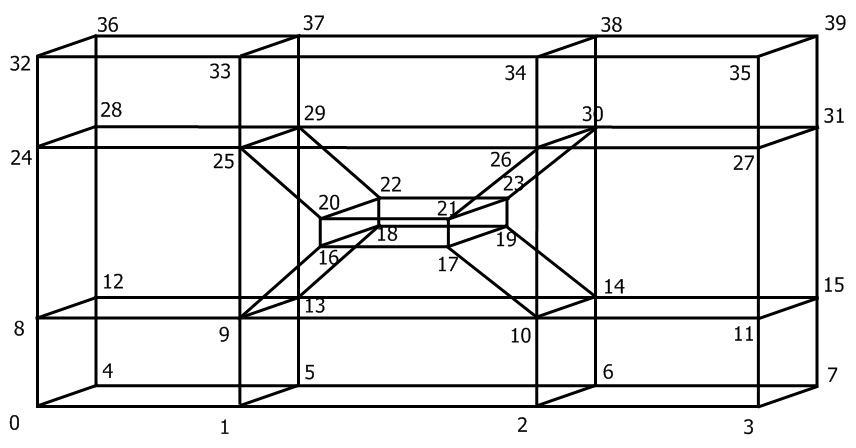
\includegraphics[width=0.95\linewidth]{openfoam-horizontal-plate.png}
\end{figure}
}

\subsection{Create mesh}
\frame{\frametitle{Create mesh}
\textbf{Create mesh using blockMesh utility:}

[user@server]\$ blockMesh -case name-of-model
\begin{figure}
   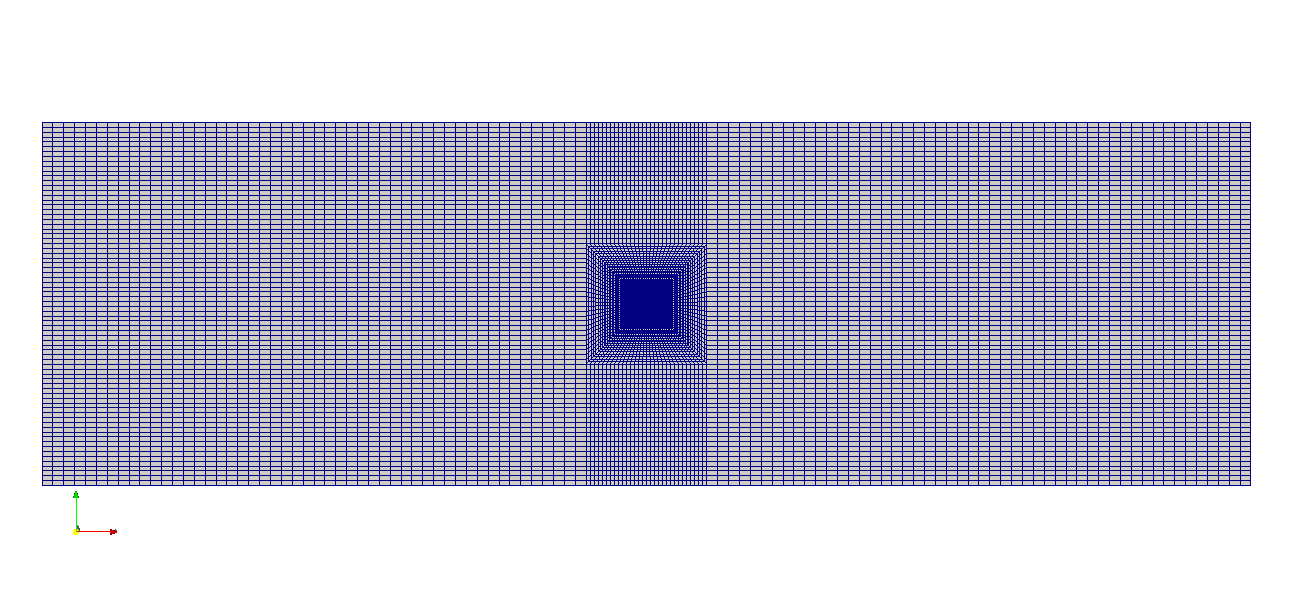
\includegraphics[width=0.99\linewidth]{grid-model.png}
\end{figure}
\textbf{Boundary conditions:}

Top, Botton, Left, Right: freeSteram (U, p), zeroGradient (S)

Plate: oscillating (U), fixedGradient (S)
}


\section{Results}

\subsection{Results of calculations. Different velocities}
\frame{\frametitle{Different velocities $L_x=1$ cm, $N=0.9\ s^{-1}$, $\omega=0.54\ s^{-1}$ \\
Module of velocity. Source - horizontal plate. Type - piston}
\begin{figure}
\begin{minipage}{0.47\linewidth}
 \center{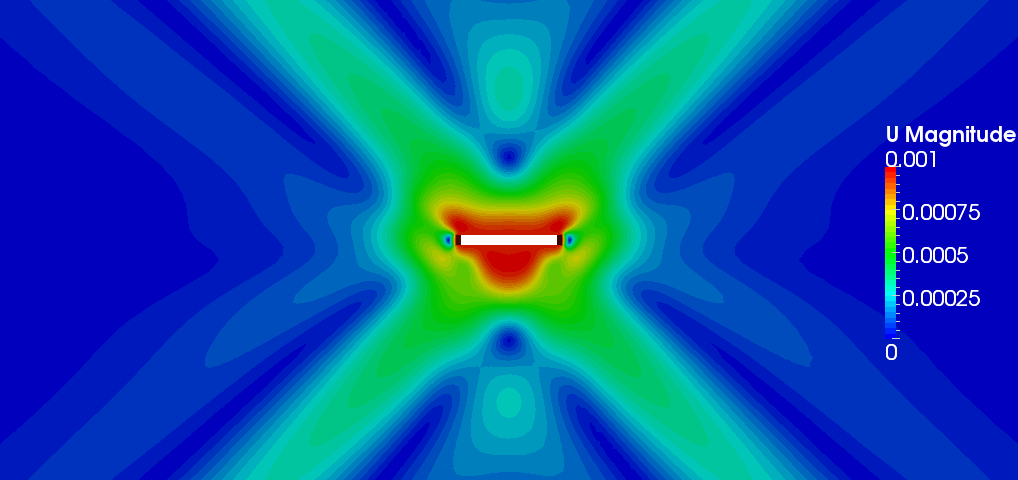
\includegraphics[width=0.8\linewidth]{results/U1E-3Umag.png}}\\
\tiny{$u_0=0.001\ m\ s^{-1}$}
\end{minipage}
\hfill
\begin{minipage}{0.47\linewidth}
 \center{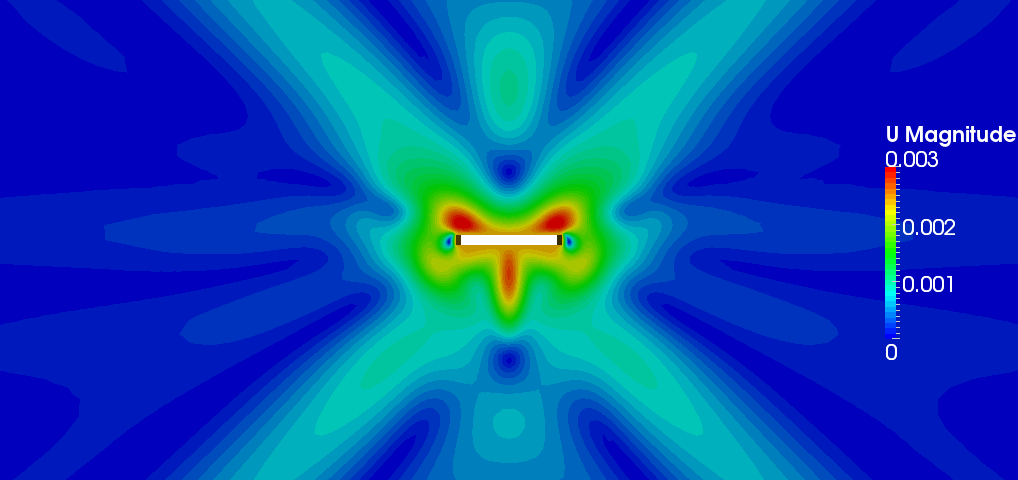
\includegraphics[width=0.8\linewidth]{results/U2_5E-3Umag.png}}\\
\tiny{$u_0=0.0025\ m\ s^{-1}$}
\end{minipage}
\vfill{}
\begin{minipage}{0.47\linewidth}
 \center{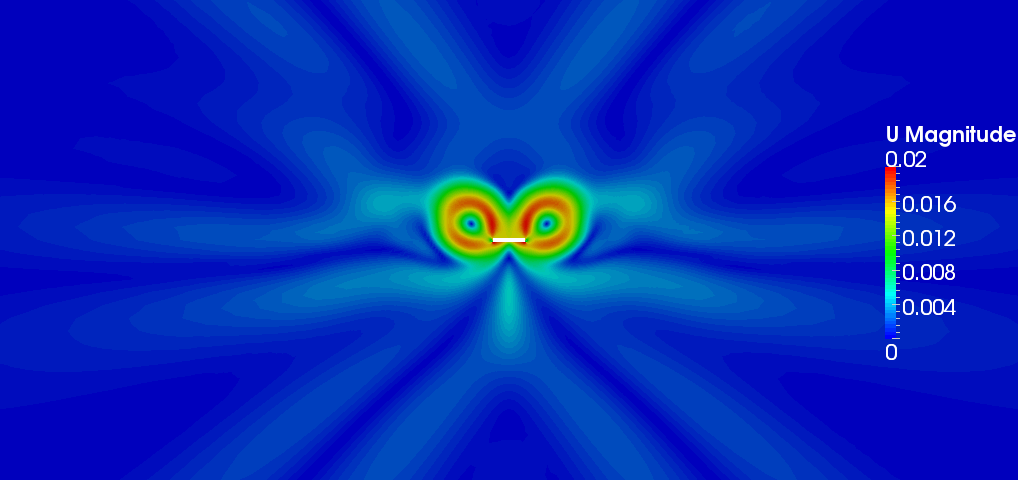
\includegraphics[width=0.8\linewidth]{results/U2_5E-2Umag.png}}\\
\tiny{$u_0=0.025\ m\ s^{-1}$}
\end{minipage}
\begin{minipage}{0.47\linewidth}
 \center{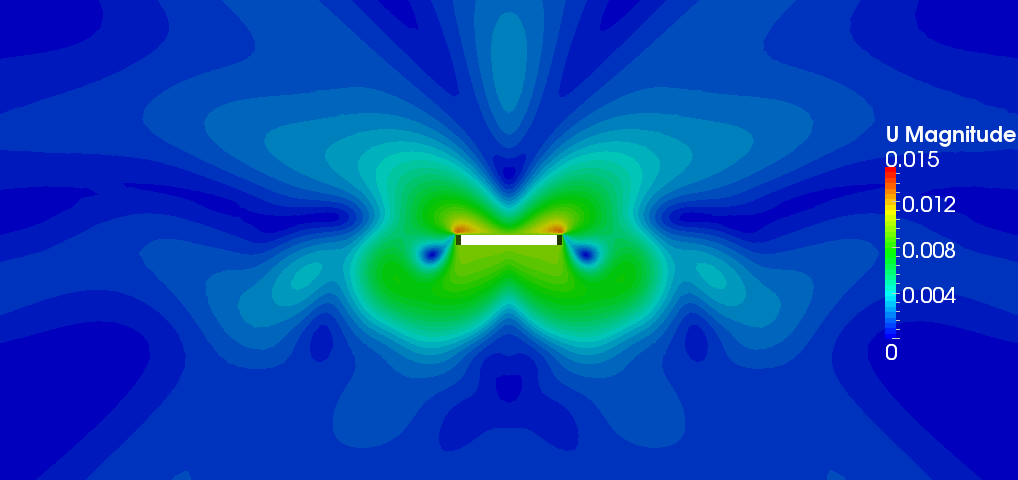
\includegraphics[width=0.8\linewidth]{results/U1E-2Umag.png}}\\
\tiny{$u_0=0.01\ m\ s^{-1}$}
\end{minipage}
\end{figure}
}


\subsection{Results of calculations. Different velocities}
\frame{\frametitle{Different velocities $L_x=1$ cm, $N=0.9\ s^{-1}$, $\omega=0.54\ s^{-1}$ \\
Module of velocity. Source - horizontal plate. Type - friction}
\begin{figure}
\begin{minipage}{0.47\linewidth}
 \center{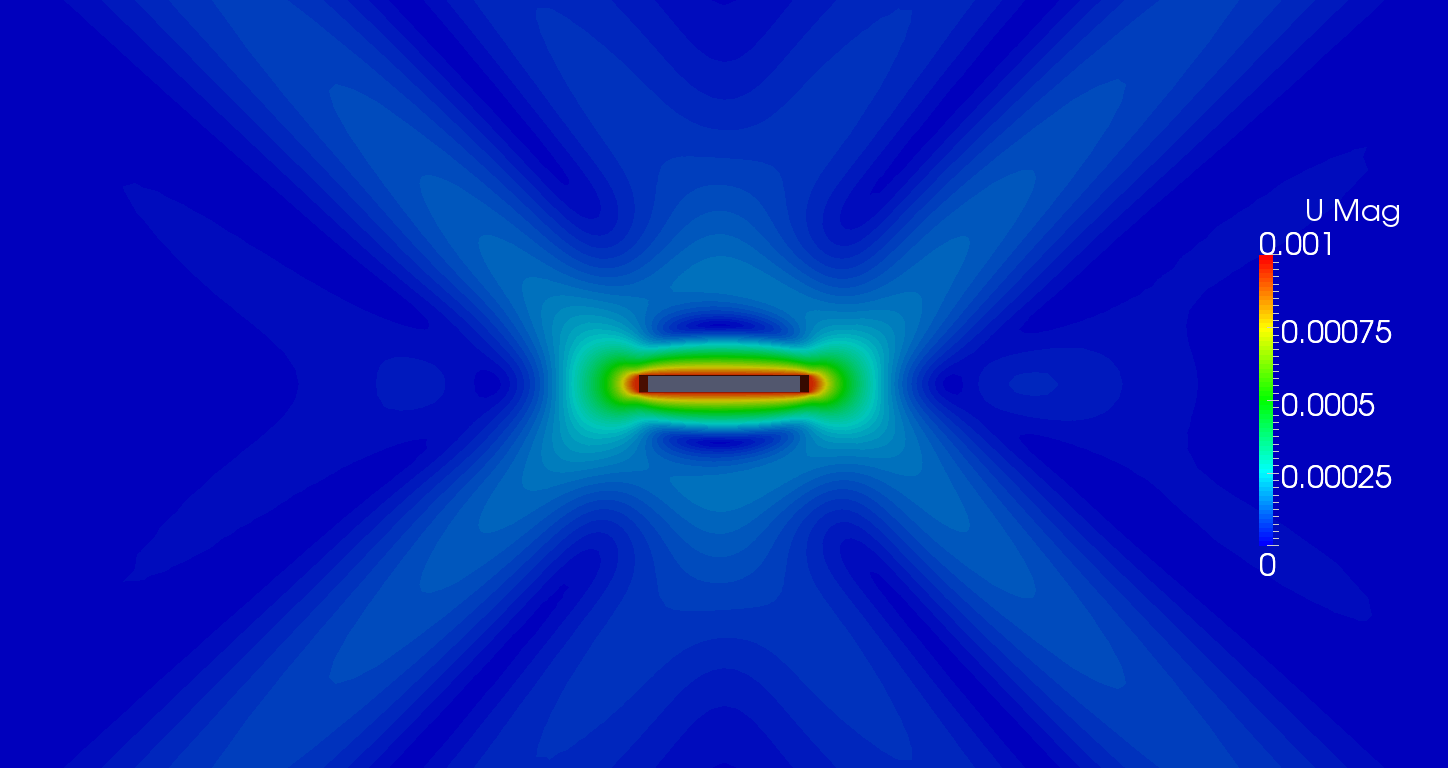
\includegraphics[width=0.8\linewidth]{results/U1E-3-fricUmag.png}}\\
\tiny{$u_0=0.001\ m\ s^{-1}$}
\end{minipage}
\hfill
\begin{minipage}{0.47\linewidth}
 \center{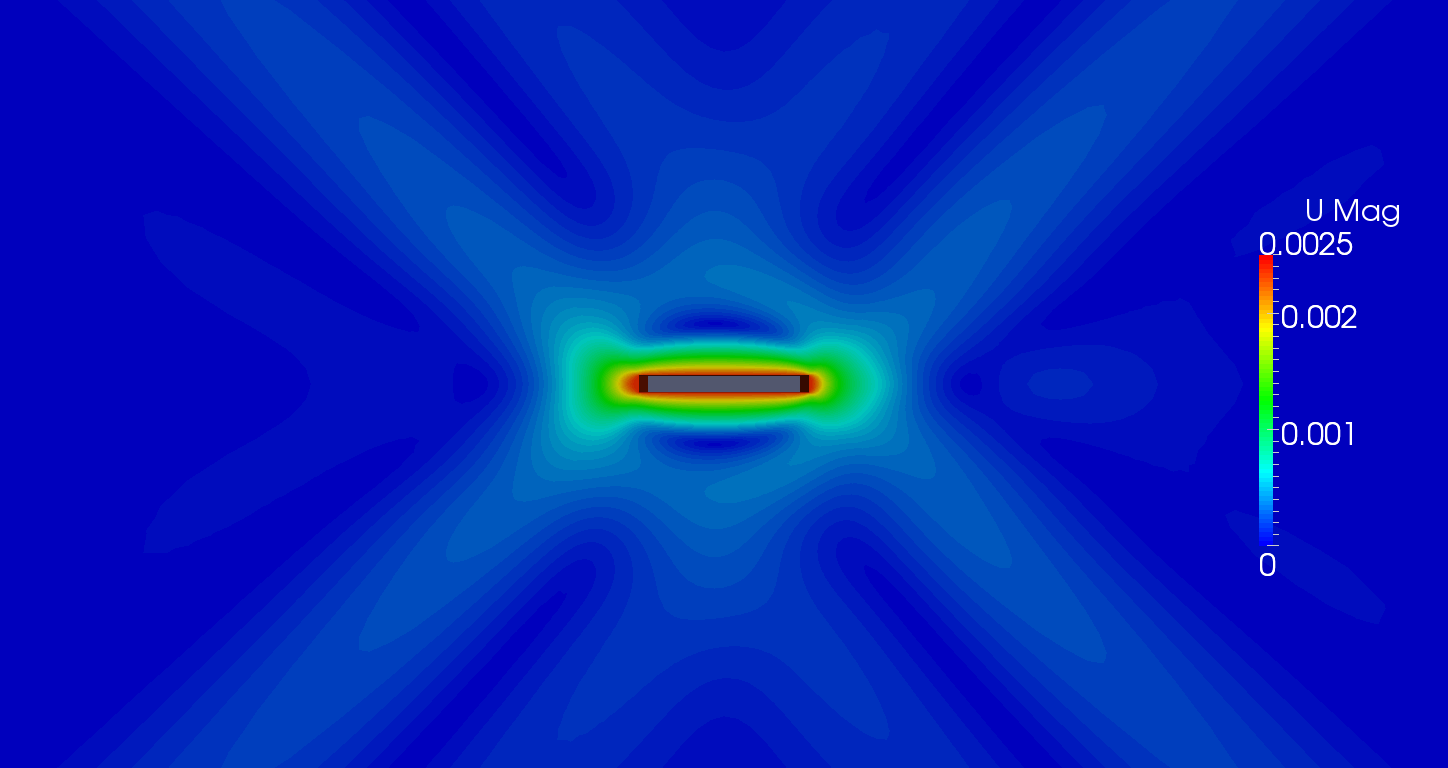
\includegraphics[width=0.8\linewidth]{results/U2_5E-3-fricUmag.png}}\\
\tiny{$u_0=0.0025\ m\ s^{-1}$}
\end{minipage}
\vfill{}
\begin{minipage}{0.47\linewidth}
 \center{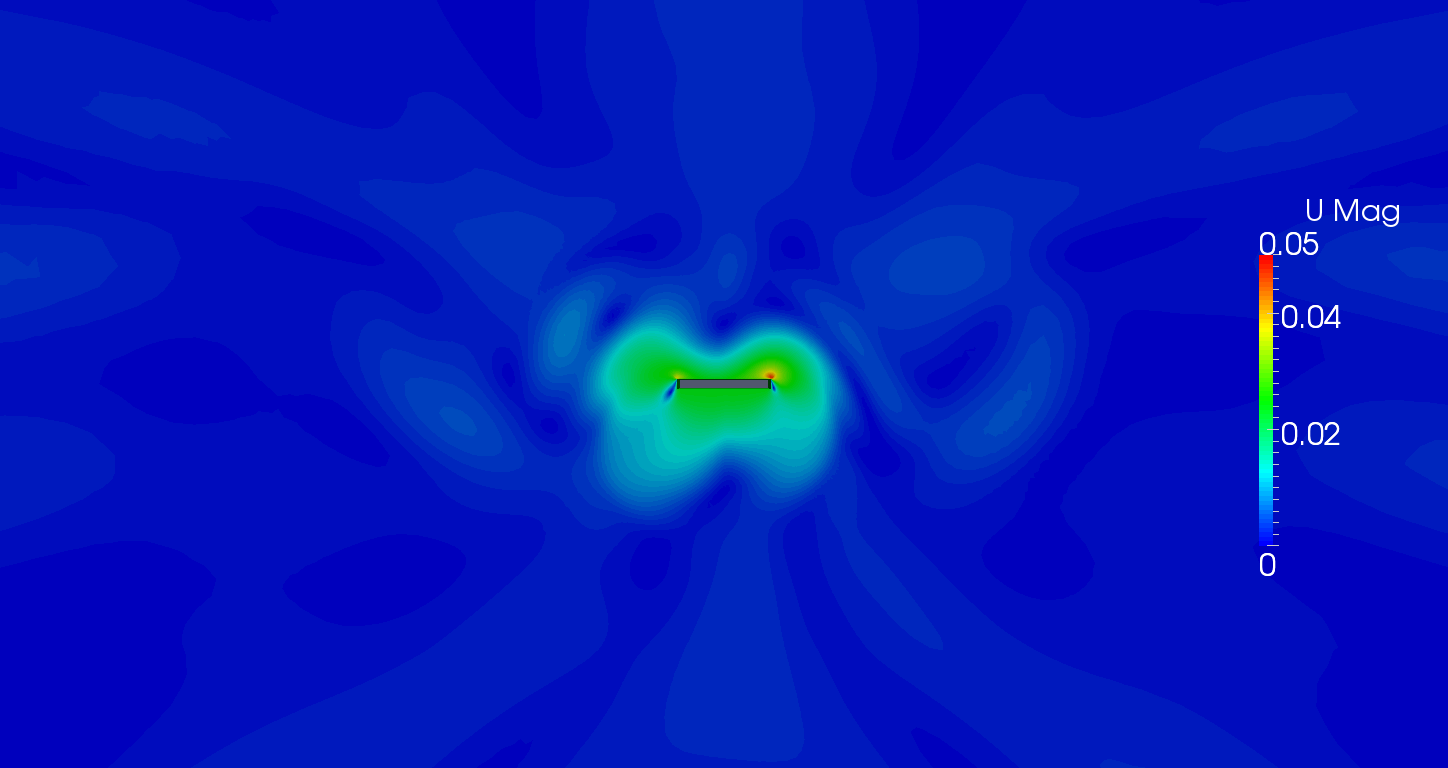
\includegraphics[width=0.8\linewidth]{results/U2_5E-2-fricUmag.png}}\\
\tiny{$u_0=0.025\ m\ s^{-1}$}
\end{minipage}
\begin{minipage}{0.47\linewidth}
 \center{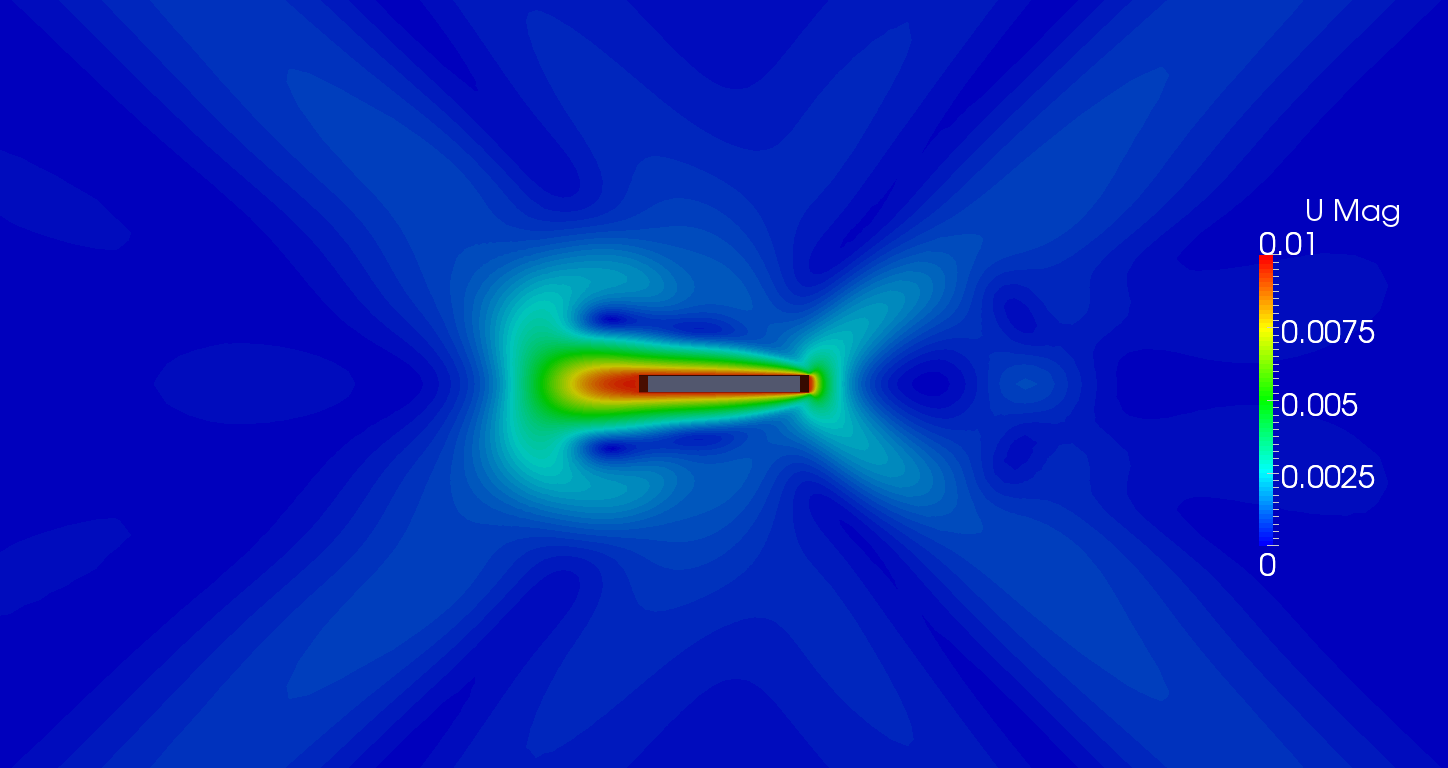
\includegraphics[width=0.8\linewidth]{results/U1E-2-fricUmag.png}}\\
\tiny{$u_0=0.01\ m\ s^{-1}$}
\end{minipage}
\end{figure}
}


% \subsection{Results of calculations. Different size of plate}
% \frame{\frametitle{Different size of plate $\nu=10^{-2}\ cm^2\ s^{-1}$, $N=0.9\ s^{-1}$, $\omega=0.54\ s^{-1}$ \\
% Module of velocity. Source - horizontal plate.}
% \begin{figure}
% \begin{minipage}{0.47\linewidth}
%  \center{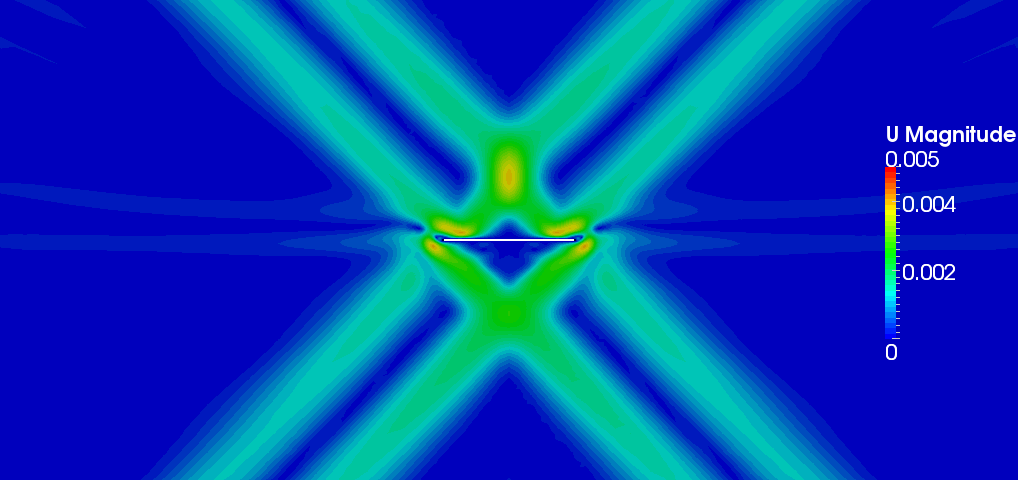
\includegraphics[width=0.8\linewidth]{Lx0_05Umag.png}}\\
% \tiny{$L_x=5 \ cm$}
% \end{minipage}
% \hfill
% \begin{minipage}{0.47\linewidth}
%  \center{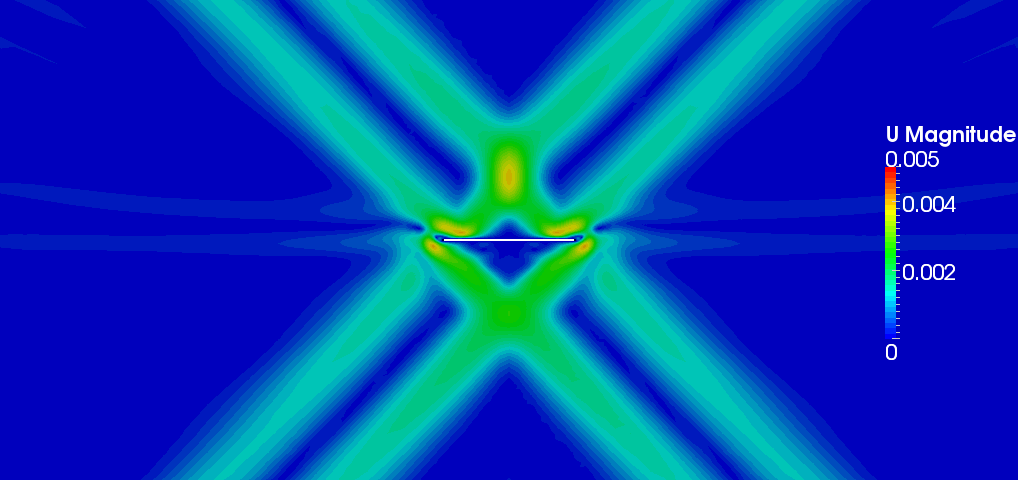
\includegraphics[width=0.8\linewidth]{Lx0_05Umag.png}}\\
% \tiny{$L_x=5 \ cm$}
% \end{minipage}
% \vfill{}
% \begin{minipage}{0.47\linewidth}
%  \center{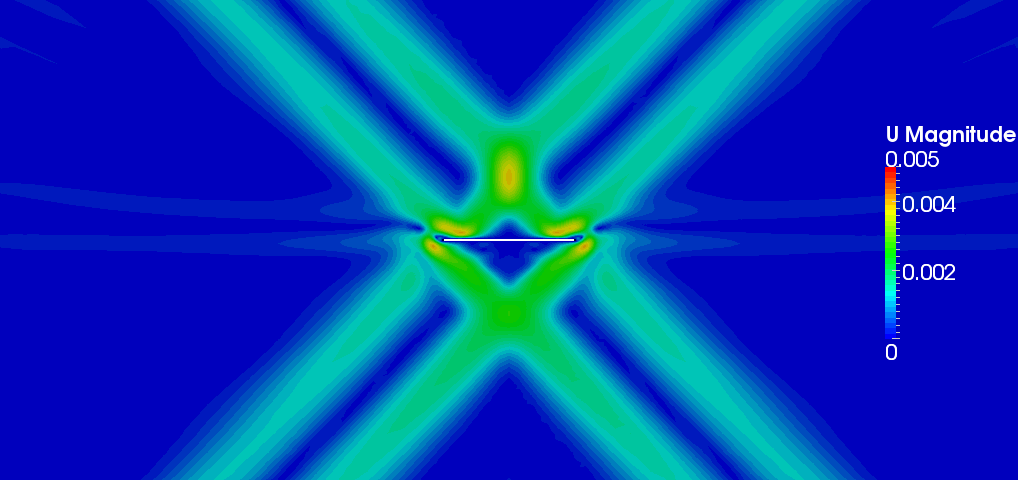
\includegraphics[width=0.8\linewidth]{Lx0_05Umag.png}}\\
% \tiny{$L_x=5 \ cm$}
% \end{minipage}
% \begin{minipage}{0.47\linewidth}
%  \center{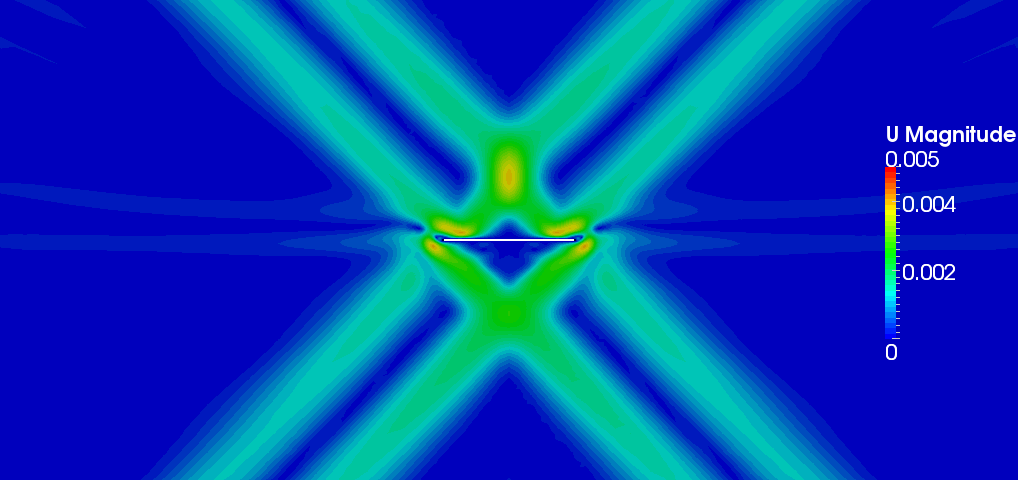
\includegraphics[width=0.8\linewidth]{Lx0_05Umag.png}}\\
% \tiny{$L_x=5 \ cm$}
% \end{minipage}
% \end{figure}
% }


\subsection{Results of calculations. Different viscosity}
\frame{\frametitle{Different viscosity $L_x=1$ cm, $N=0.9\ s^{-1}$, $\omega=0.54\ s^{-1}$ \\
Module of velocity. Source - horizontal plate. Type - piston}
\begin{figure}
\begin{minipage}{0.47\linewidth}
 \center{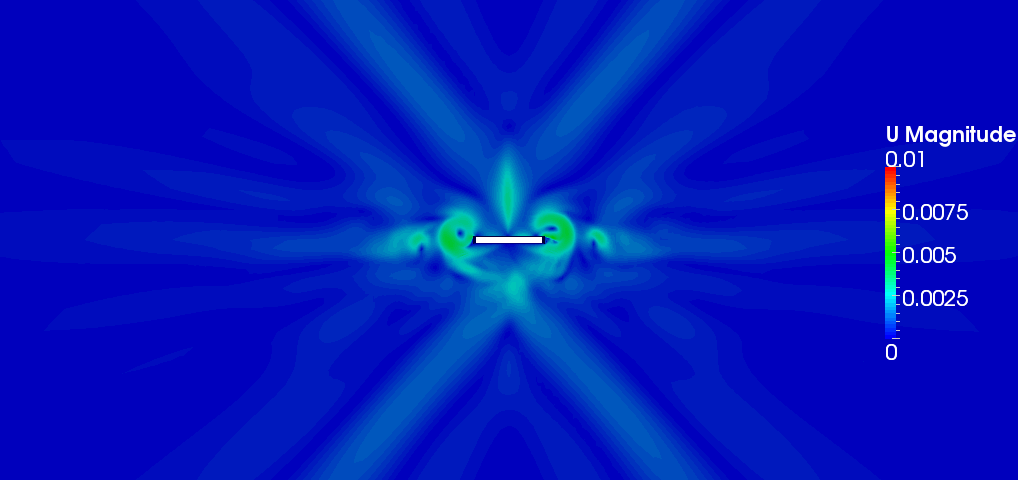
\includegraphics[width=0.8\linewidth]{results/nu10E-9Umag.png}}\\
\tiny{$\nu=10^{-8}\ m^2\ s^{-1}$}
\end{minipage}
\hfill
\begin{minipage}{0.47\linewidth}
 \center{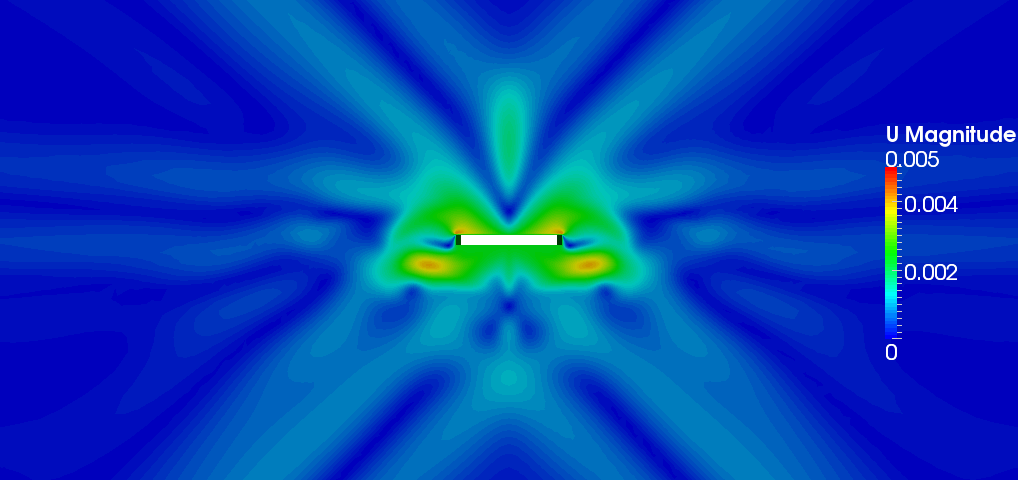
\includegraphics[width=0.8\linewidth]{results/nu10E-7Umag.png}}\\
\tiny{$\nu=10^{-7}\ m^2\ s^{-1}$}
\end{minipage}
\vfill{}
\begin{minipage}{0.47\linewidth}
 \center{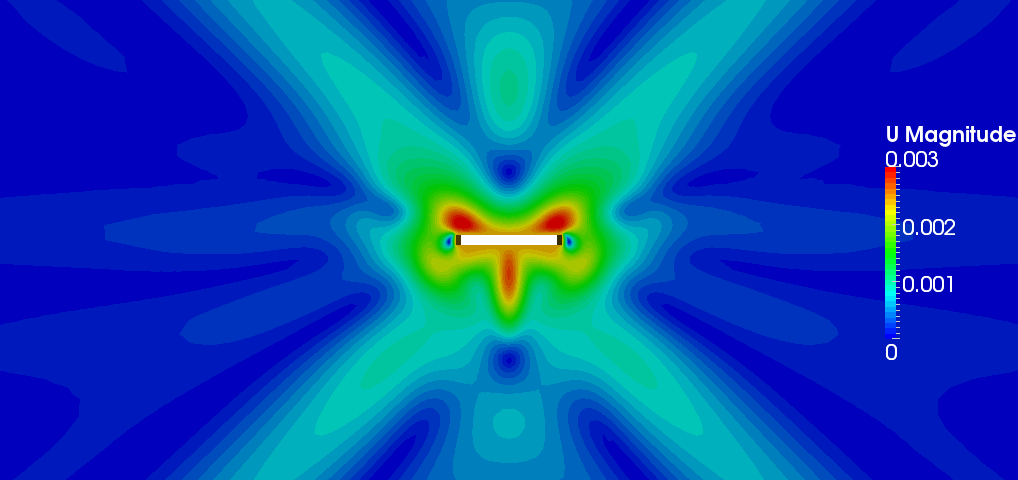
\includegraphics[width=0.8\linewidth]{results/U2_5E-3Umag.png}}\\
\tiny{$\nu=10^{-6}\ m^2\ s^{-1}$}
\end{minipage}
\begin{minipage}{0.47\linewidth}
 \center{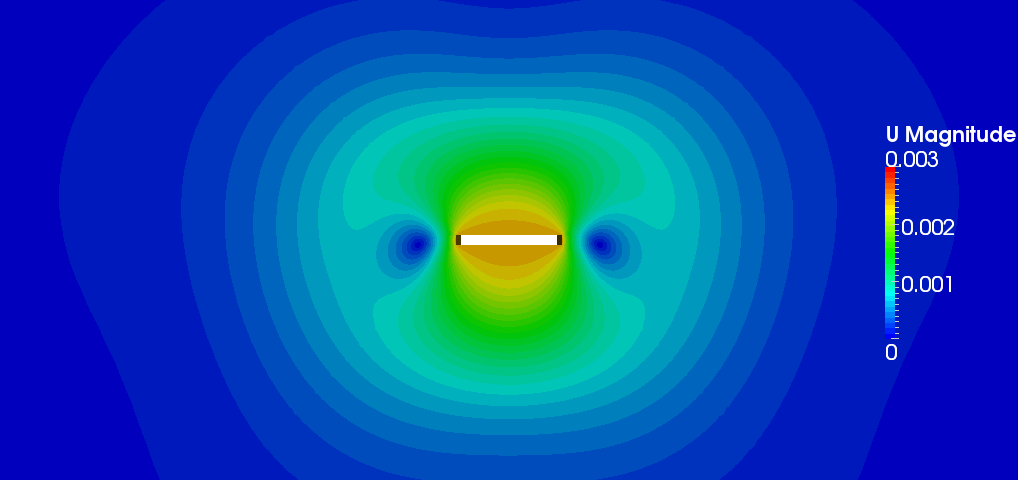
\includegraphics[width=0.8\linewidth]{results/nu10E-5Umag.png}}\\
\tiny{$\nu=10^{-5}\ m^2\ s^{-1}$}
\end{minipage}
\end{figure}
}


\subsection{Results of calculations. Different viscosity}
\frame{\frametitle{Different viscosity $L_x=1$ cm, $N=0.9\ s^{-1}$, $\omega=0.54\ s^{-1}$ \\
Module of velocity. Source - horizontal plate. Type - friction}
\begin{figure}
\begin{minipage}{0.47\linewidth}
 \center{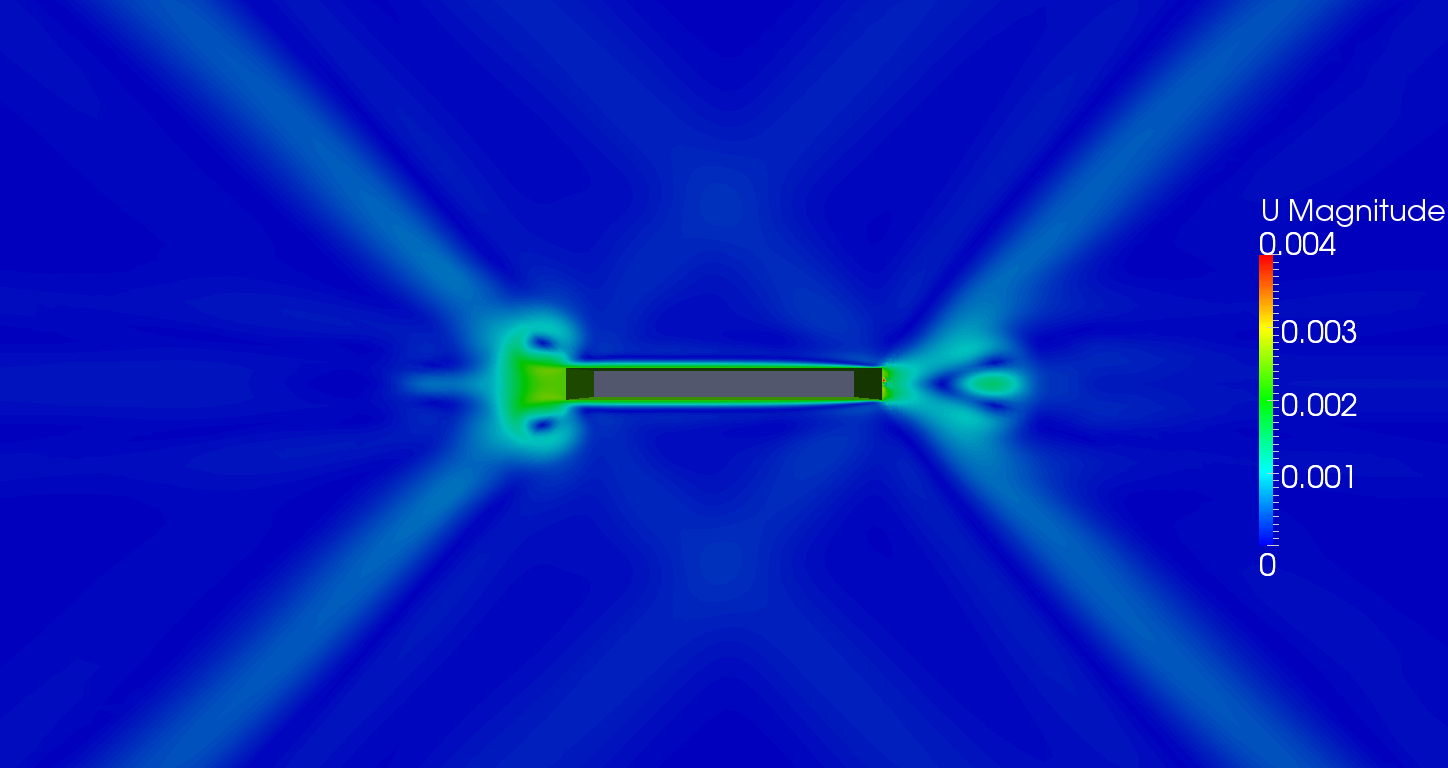
\includegraphics[width=0.8\linewidth]{results/nu10E-9-fricUmag.png}}\\
\tiny{$\nu=10^{-8}\ m^2\ s^{-1}$}
\end{minipage}
\hfill
\begin{minipage}{0.47\linewidth}
 \center{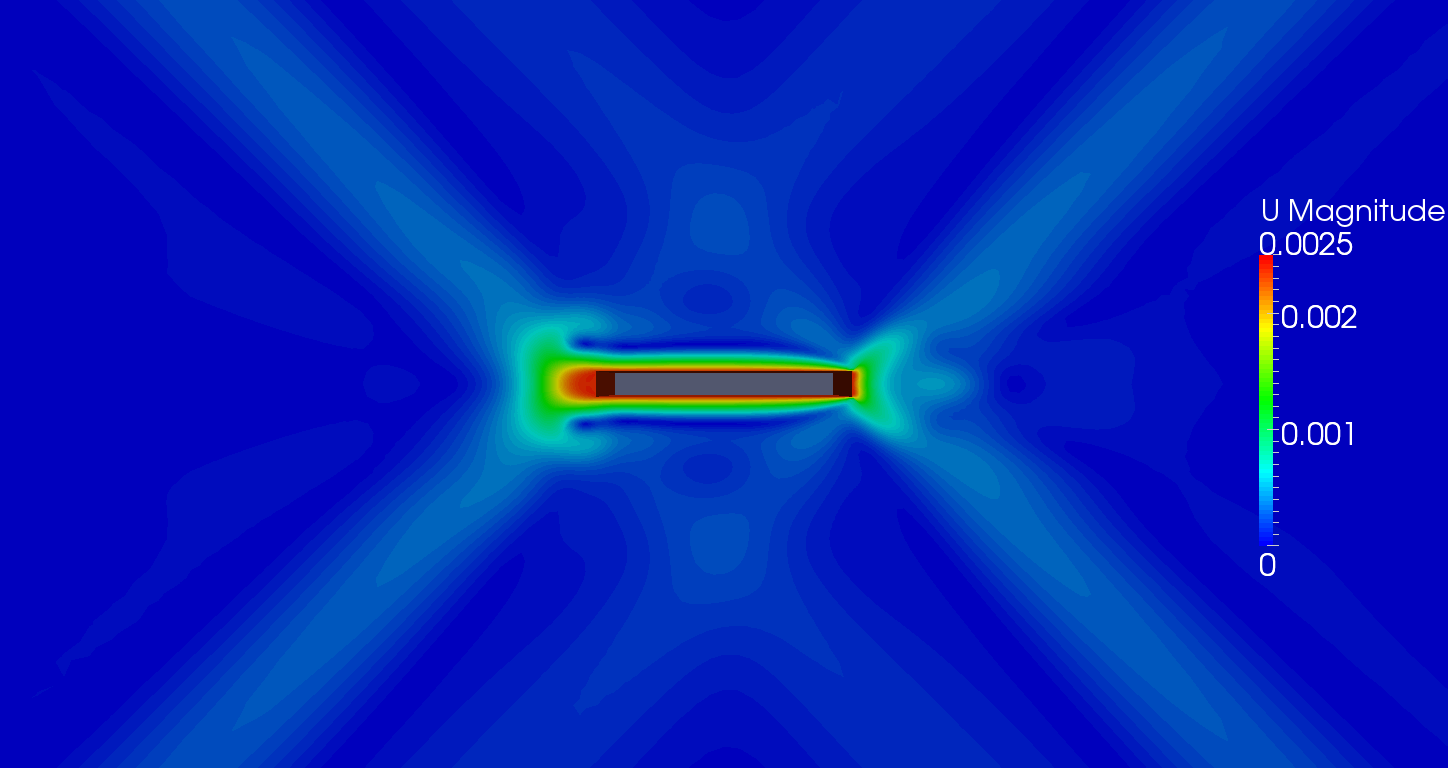
\includegraphics[width=0.8\linewidth]{results/nu10E-7-fricUmag.png}}\\
\tiny{$\nu=10^{-7}\ m^2\ s^{-1}$}
\end{minipage}
\vfill{}
\begin{minipage}{0.47\linewidth}
 \center{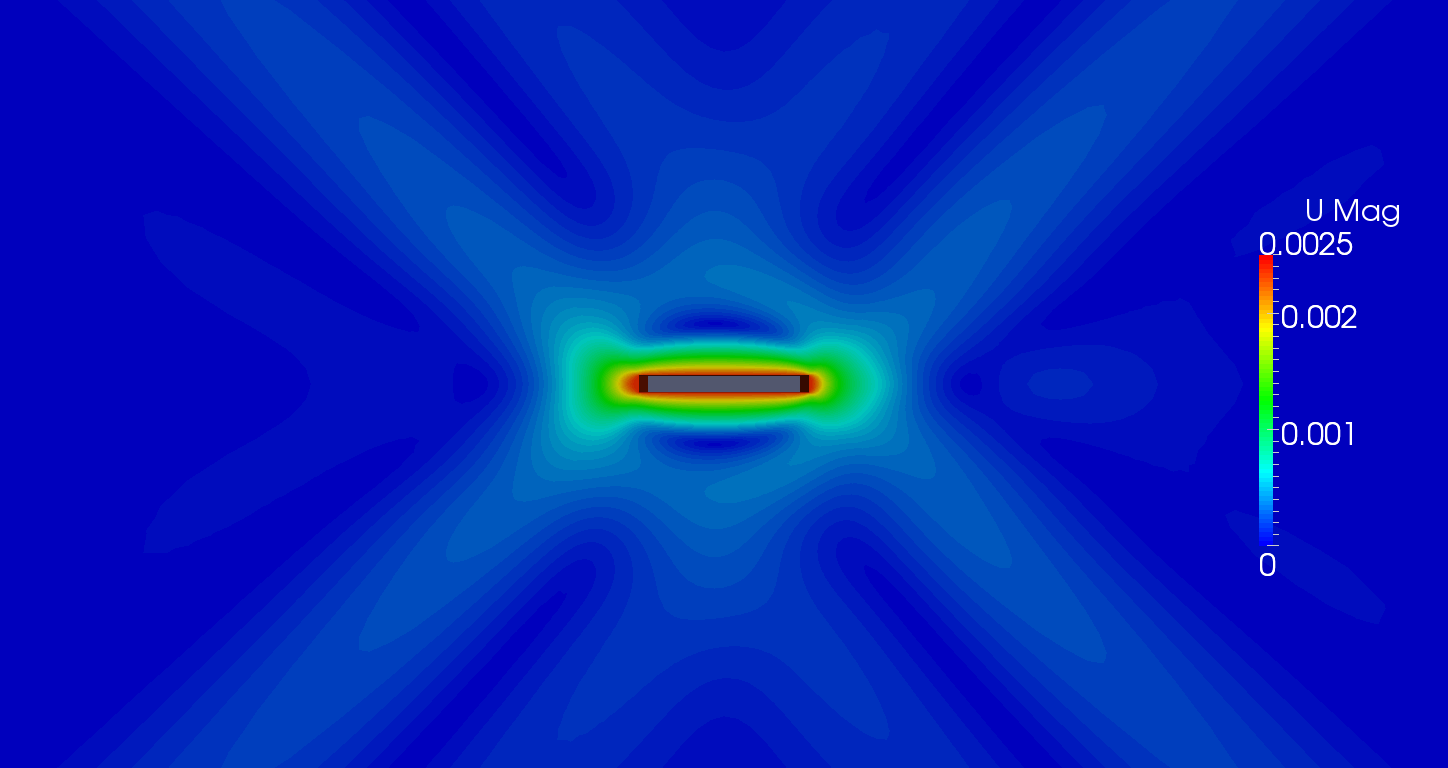
\includegraphics[width=0.8\linewidth]{results/U2_5E-3-fricUmag.png}}\\
\tiny{$\nu=10^{-6}\ m^2\ s^{-1}$}
\end{minipage}
\begin{minipage}{0.47\linewidth}
 \center{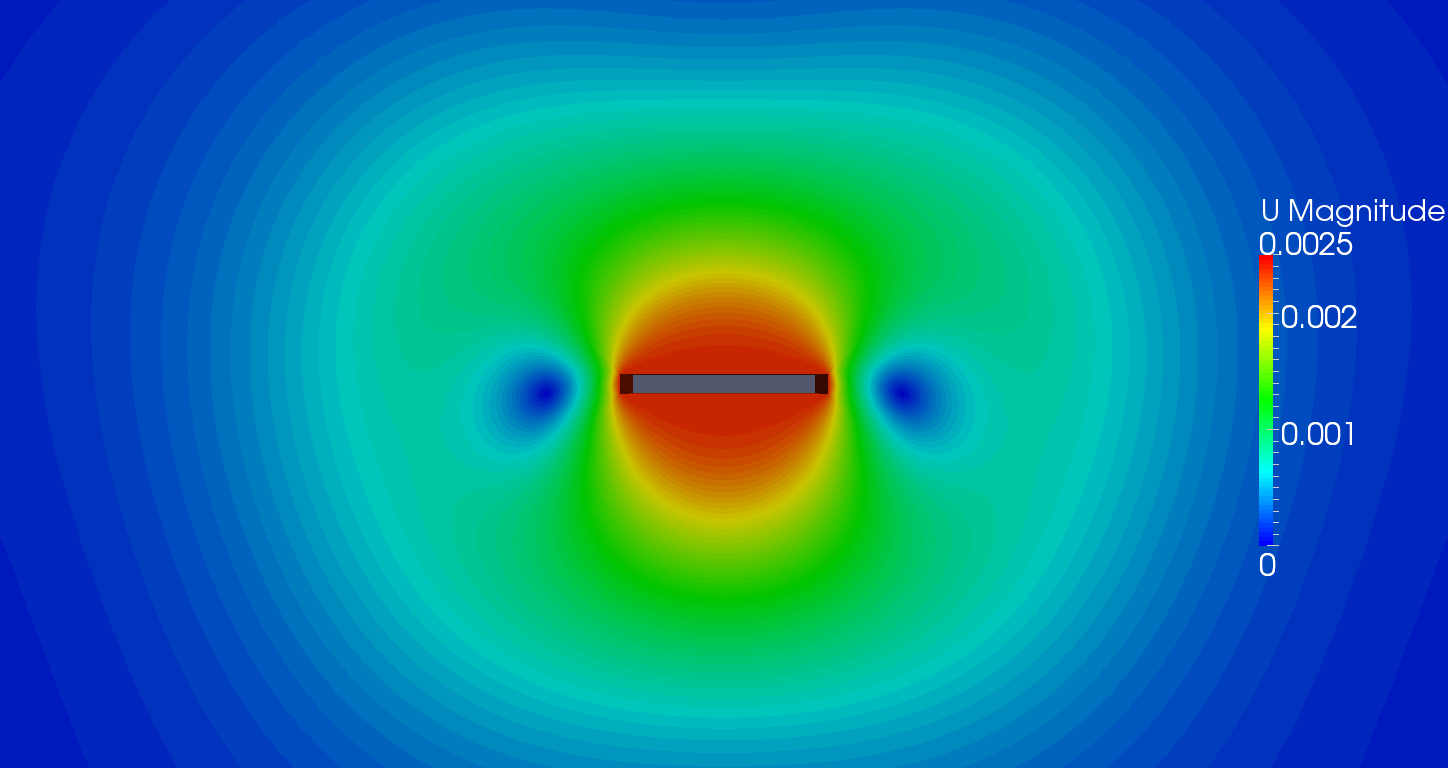
\includegraphics[width=0.8\linewidth]{results/nu10E-5-fricUmag.png}}\\
\tiny{$\nu=10^{-5}\ m^2\ s^{-1}$}
\end{minipage}
\end{figure}
}

\subsection{Results of calculations. Different stratification}
\frame{\frametitle{Different stratification $L_x=1$ cm, $\nu=10^{-2}\ cm^2\ s^{-1}$, $\omega=0.54\ s^{-1}$ \\
Module of velocity. Source - horizontal plate. Type - piston}
\begin{figure}
\begin{minipage}{0.47\linewidth}
 \center{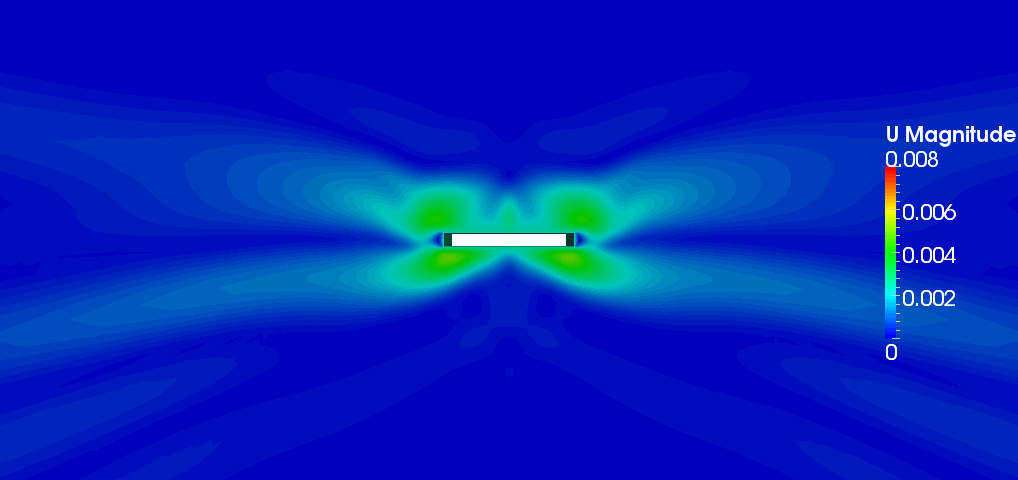
\includegraphics[width=0.8\linewidth]{results/N=2_8Umag.png}}\\
\tiny{$N=2.8\ s^{-1}$}
\end{minipage}
\hfill
\begin{minipage}{0.47\linewidth}
 \center{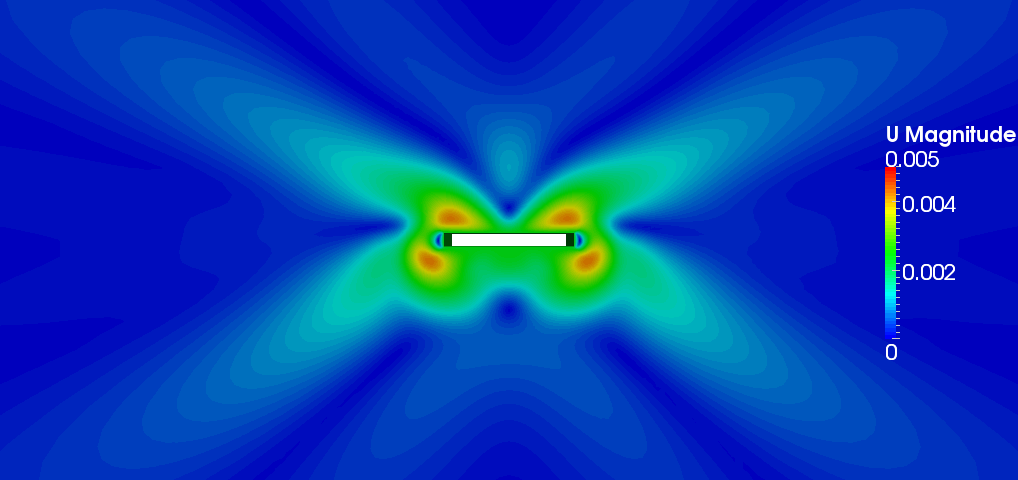
\includegraphics[width=0.74\linewidth]{results/N=1_46Umag.png}}\\
\tiny{$N=1.46\ s^{-1}$}
\end{minipage}
\vfill{}
\begin{minipage}{0.47\linewidth}
 \center{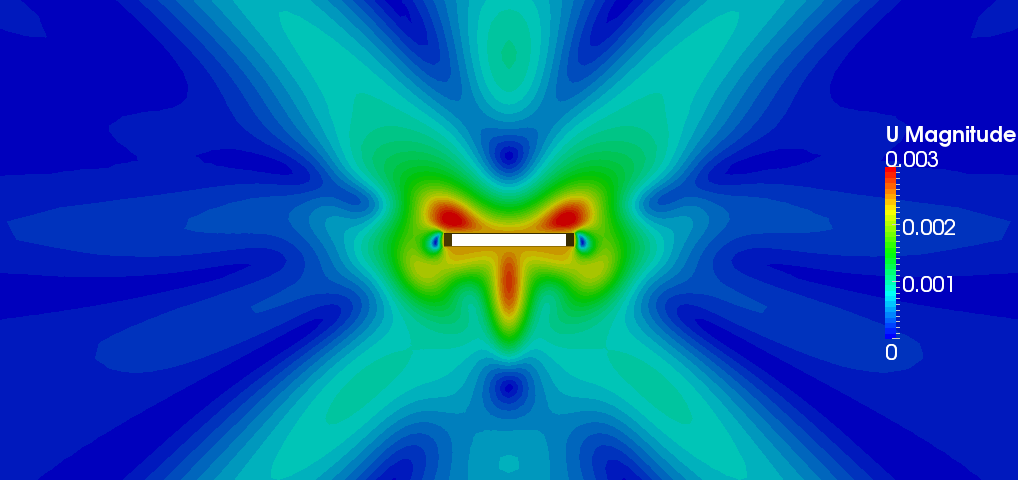
\includegraphics[width=0.8\linewidth]{results/N=0_7Umag.png}}\\
\tiny{$N=2.8\ s^{-1}$}
\end{minipage}
\begin{minipage}{0.47\linewidth}
 \center{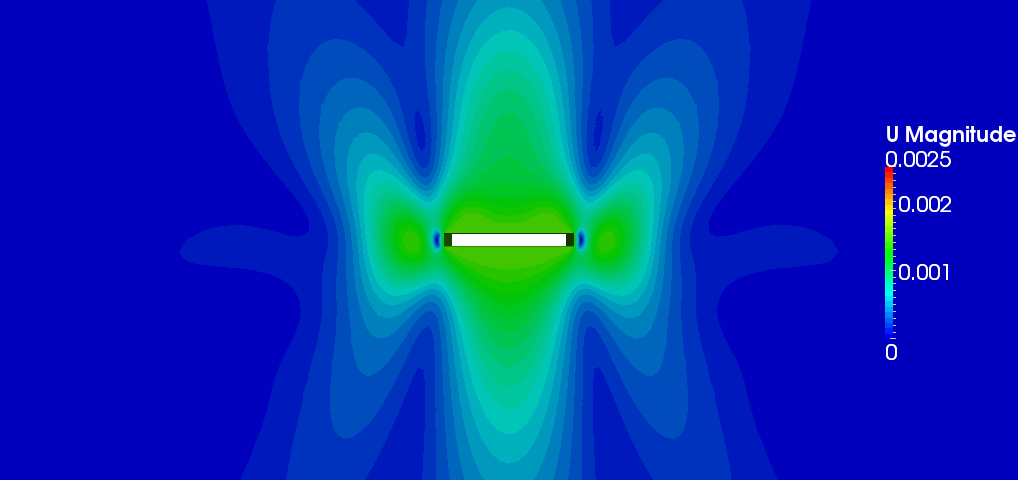
\includegraphics[width=0.8\linewidth]{results/N=0_58Umag.png}}\\
\tiny{$N=0.58\ s^{-1}$}
\end{minipage}
\end{figure}
}

\subsection{Results of calculations. Different stratification}
\frame{\frametitle{Different stratification $L_x=1$ cm, $\nu=10^{-2}\ cm^2\ s^{-1}$, $\omega=0.54\ s^{-1}$ \\
Module of velocity. Source - horizontal plate. Type - friction}
\begin{figure}
\begin{minipage}{0.47\linewidth}
 \center{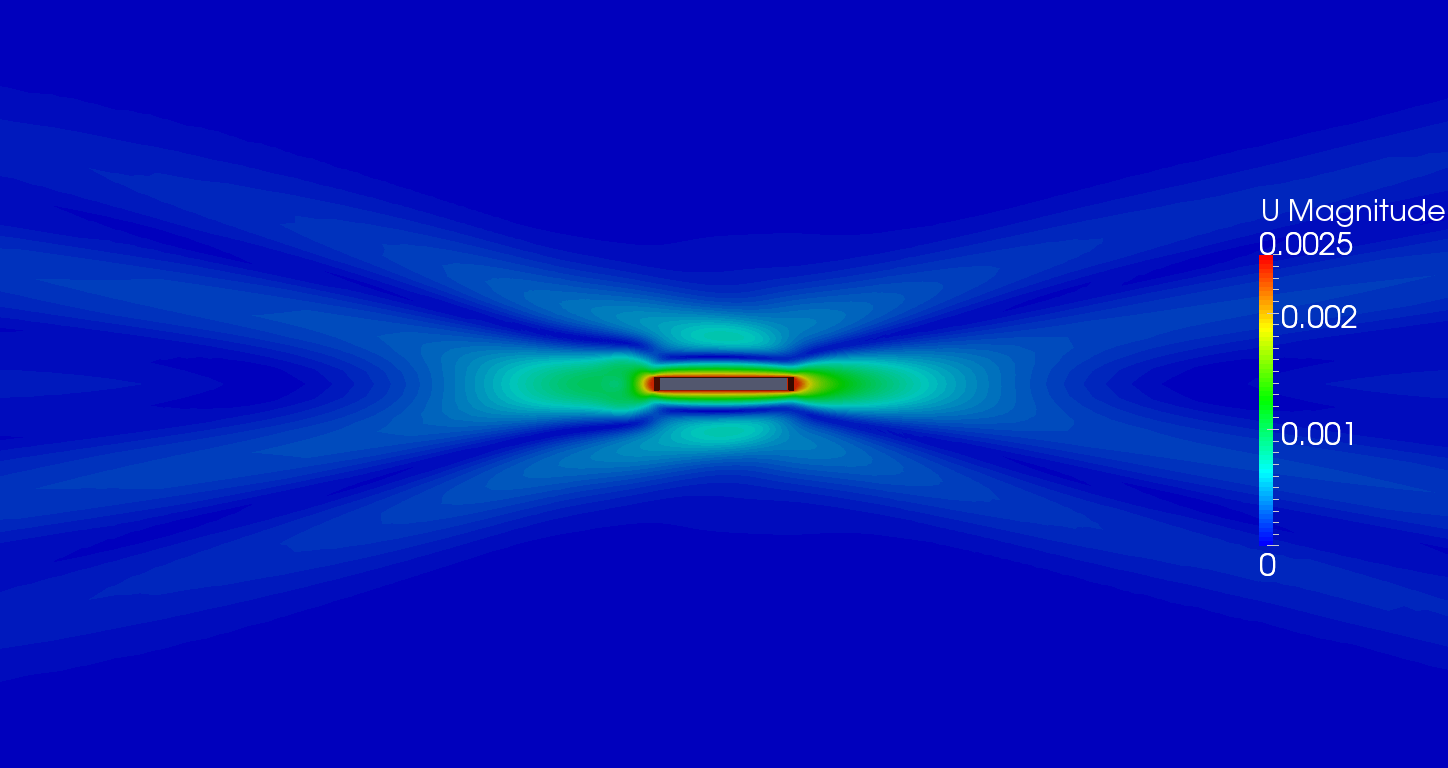
\includegraphics[width=0.8\linewidth]{results/N=2_8-fricUmag.png}}\\
\tiny{$N=2.8\ s^{-1}$}
\end{minipage}
\hfill
\begin{minipage}{0.47\linewidth}
 \center{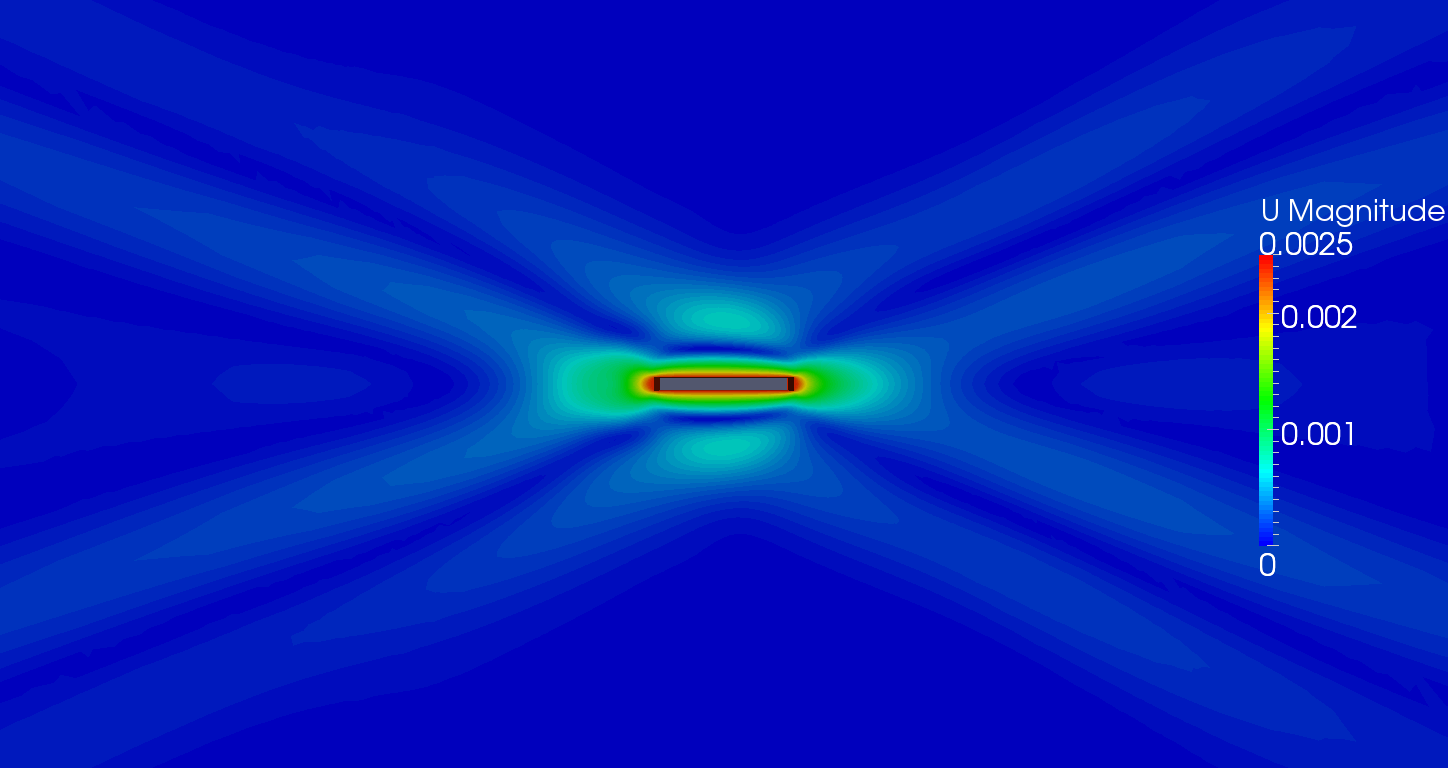
\includegraphics[width=0.74\linewidth]{results/N=1_46-fricUmag.png}}\\
\tiny{$N=1.46\ s^{-1}$}
\end{minipage}
\vfill{}
\begin{minipage}{0.47\linewidth}
 \center{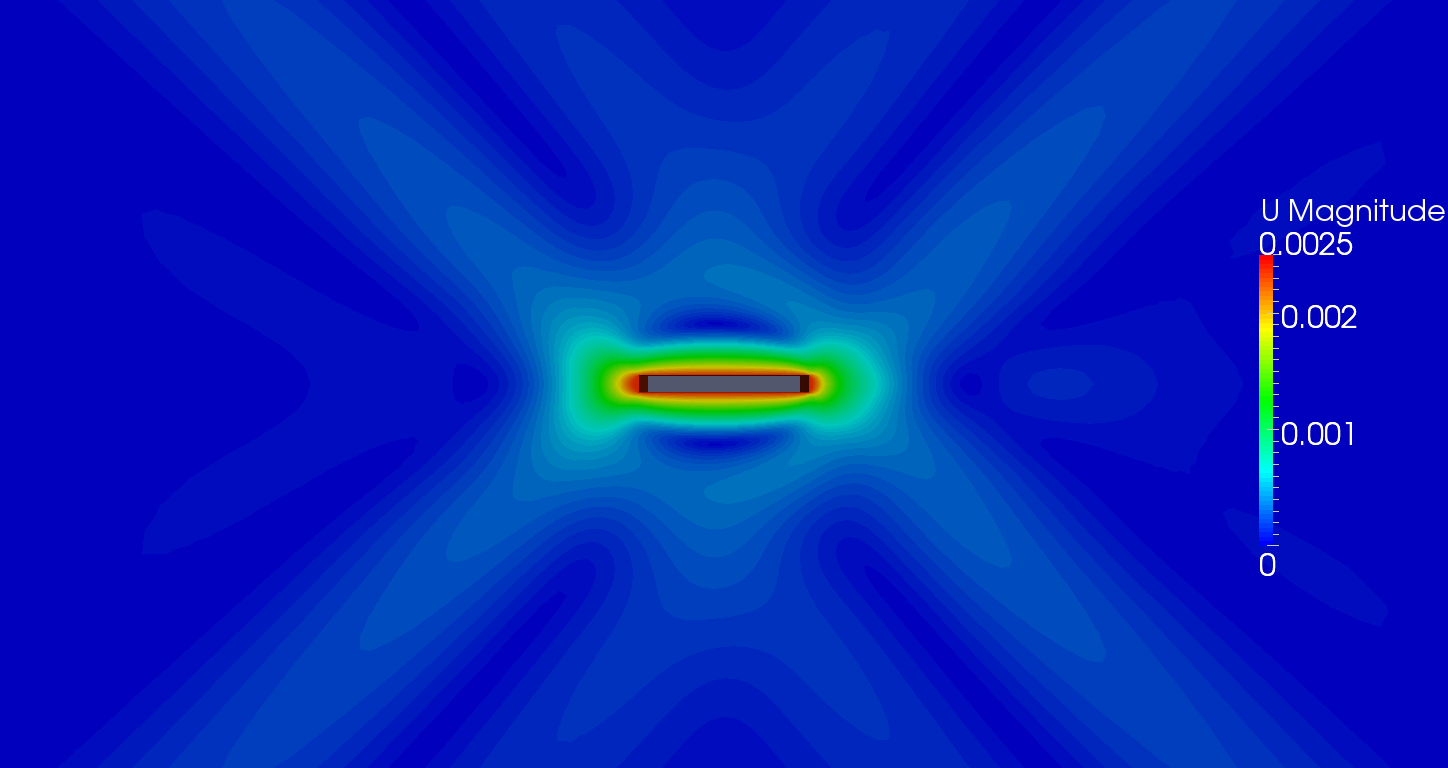
\includegraphics[width=0.8\linewidth]{results/N=0_7-fricUmag.png}}\\
\tiny{$N=2.8\ s^{-1}$}
\end{minipage}
\begin{minipage}{0.47\linewidth}
 \center{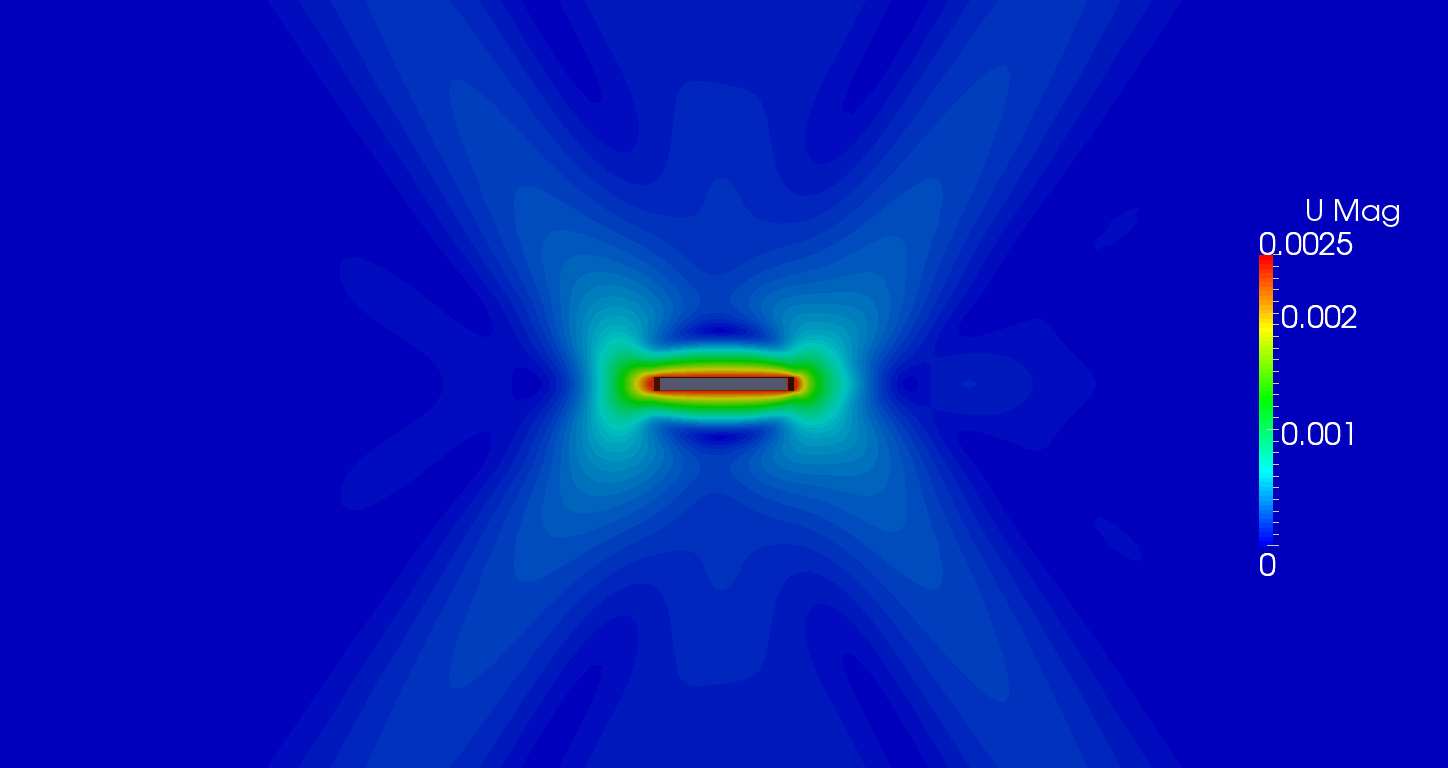
\includegraphics[width=0.8\linewidth]{results/N=0_58-fricUmag.png}}\\
\tiny{$N=0.58\ s^{-1}$}
\end{minipage}
\end{figure}
}

\section{Conclusion}
\frame{\frametitle{Conclusion}
\begin{enumerate}
\item 
In the general case, in a viscous stratified fluid there are two types of solutions:
regular (waves) and three type singular solutions. Two of them don't have analogues in homogeneous fluid 
Their properties are defined viscosity, stratification, diffusion and the geometry of the problem;
\item For a complete description of the flow of fluid you must consider all parameters (viscosity,
stratification diffusion);
\item Create solver for calculation of the internal gravity waves in a continuesly stratified fluid;
\item Calculations case horizontal plate.
\end{enumerate}
}

\end{document} 